% Create a beamer file with cool style.

\documentclass{beamer}
\usetheme{Madrid}
\usecolortheme{seahorse}
\usefonttheme{serif}
\useinnertheme{rectangles}
\useoutertheme{infolines}

% We present in english
%\usepackage[swedish]{babel}
\usepackage[utf8]{inputenc}
\usepackage{
	listings,
    pgfgantt,
    xspace,
    xstring,
}

\newcommand{\stoe}{S$^2$E\xspace}

\begin{document}
\year=2023
\month=5
\day=26

\title{AMBA}
\subtitle{Interaktiv visualisering av symbolisk fuzzing}
\author{
	\mbox{Loke Gustafsson} \and
	\mbox{Samuel Kyletoft} \and
	\mbox{Enayatullah Norozi} \and
	\mbox{Albin Otterhäll} \and
	\mbox{Clara Salberg} \and
	\mbox{Linus Wallman}
}
\date{\today}

\frame{\titlepage}


% 1. (minut 1) Motivera behovet att analysera en binär (saknar källkod,
% kompilatorbuggar, ditt språk har sämst tooling)
\begin{frame}
	\frametitle{hello world}

	hello world
\end{frame}


% 2. (minut 2-3) Förklara några binäranalysmetoder (debugger, fuzzing)

\begin{frame}
	% Some examples of binary analysis methods are: 
	% binary debugging, which might be a little too manual in many cases;

	% Studying disassembly or decompiling using heuristics and meta data to
	% generate a higher level pseudocode;

	% fuzzing, generating different inputs and studying the outcome of the
	% program, like a crash;

	% Symbolic fuzzing, which we will get to.

	% All methods have their pros and cons and are applicable in different situations.
	% Binary debugging and studying disassembly or decompilation could be very
	% manual and burdenful for the analyst, but it could also give a very good
	% abstract understanding of the program.

	% Fuzzing is an automatic method and requires no interaction, but it doesn't
	% give any abstract understanding of the program. Only determining some
	% inputs satisfying user defined objectives. Like determining crashes,
	% detecting memory leaks and so on.

	% Another problem with fuzzing is the testcase generation. It is not trivial
	% how to generate test cases which effectively covers a large set of
	% execution paths so that no same paths are unneccessarily tested multiple
	% times, or reachable paths that were not explored.

	% The specific problem of test case generation is solved by symbolic fuzzing
	% which relies on symbolic execution.

	\begin{columns}[t]
		\begin{column}{0.5\textwidth}
			\begin{itemize}
				\item Binary debugging
				\item Disassembly
				\item Decompilation
				\item Fuzzing
				\item Symbolic fuzzing
			\end{itemize}
		\end{column}
		\begin{column}{0.5\textwidth}
			
\includegraphics[width=0.3\textwidth]{assets/GDB_Archer_Fish_by_Andreas_Arnez.svg.png}
			\footnote{\tiny by Andreas Arnez, \href{https://creativecommons.org/licenses/by-sa/3.0/us/deed.en}{CC BY-SA 3.0 us}}

			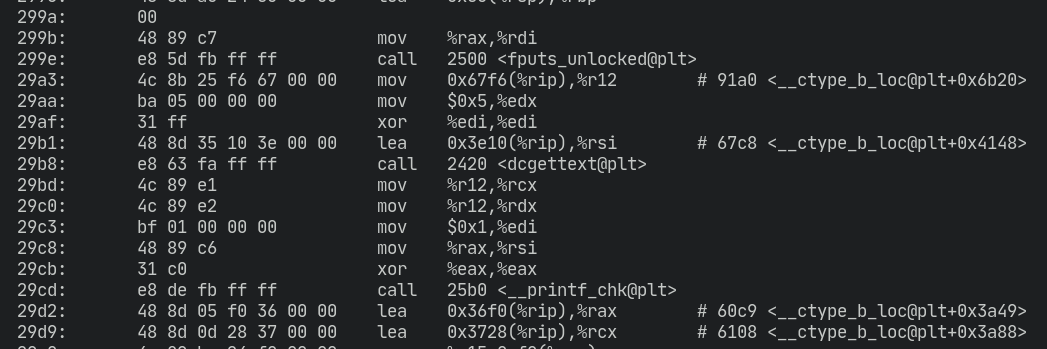
\includegraphics[width=\textwidth]{assets/disassembly.png}

			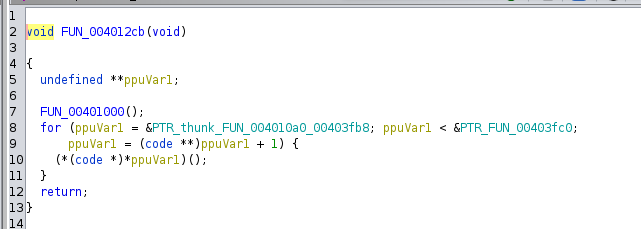
\includegraphics[width=\textwidth]{assets/decompil.png}

			\tiny{
				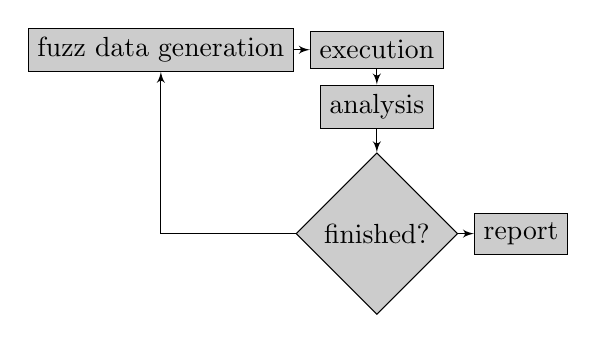
\begin{tikzpicture}

					\node [draw, fill=lightgray!80, minimum height=0.3cm]
					(first) {fuzz data generation};

					\node [draw, fill=lightgray!80, minimum height=0.3cm, right=0.2cm of first]
					(second) {execution};

					\node [draw, fill=lightgray!80, minimum height=0.3cm, below=0.2cm of second]
					(third) {analysis};

					\node [diamond, draw, fill=lightgray!80, minimum height=0.1cm, below=0.3cm of third]
					(fourth) {finished?};

					\node [draw, fill=lightgray!80, minimum height=0.3cm, right=0.2cm of fourth]
					(fifth) {report};

					\path [draw, -latex'] (first) to (second);
					\path [draw, -latex'] (second) to (third);
					\path [draw, -latex'] (third) to (fourth);
					\path [draw, -latex'] (fourth) to (fifth);
					\path [draw, -latex'] (fourth) -| (first);

				\end{tikzpicture}
			}
		\end{column}
	\end{columns}
\end{frame}


% 3. (minut 4) Förklara symbolisk exekvering
\begin{frame}
			\textbf{Symbolic Fuzzing}
	        \vspace{1.8mm}
			\small
			\begin{itemize}
				\item Explore execution paths
				\item Symbolic representation
				\item Tracking conditions into symbolic expressions
				\item Reduces the number of testcases needed
			\end{itemize}
\end{frame}

\begin{frame}
    \vspace{3.0mm}
    \textbf{State explosion}
    \begin{center}
        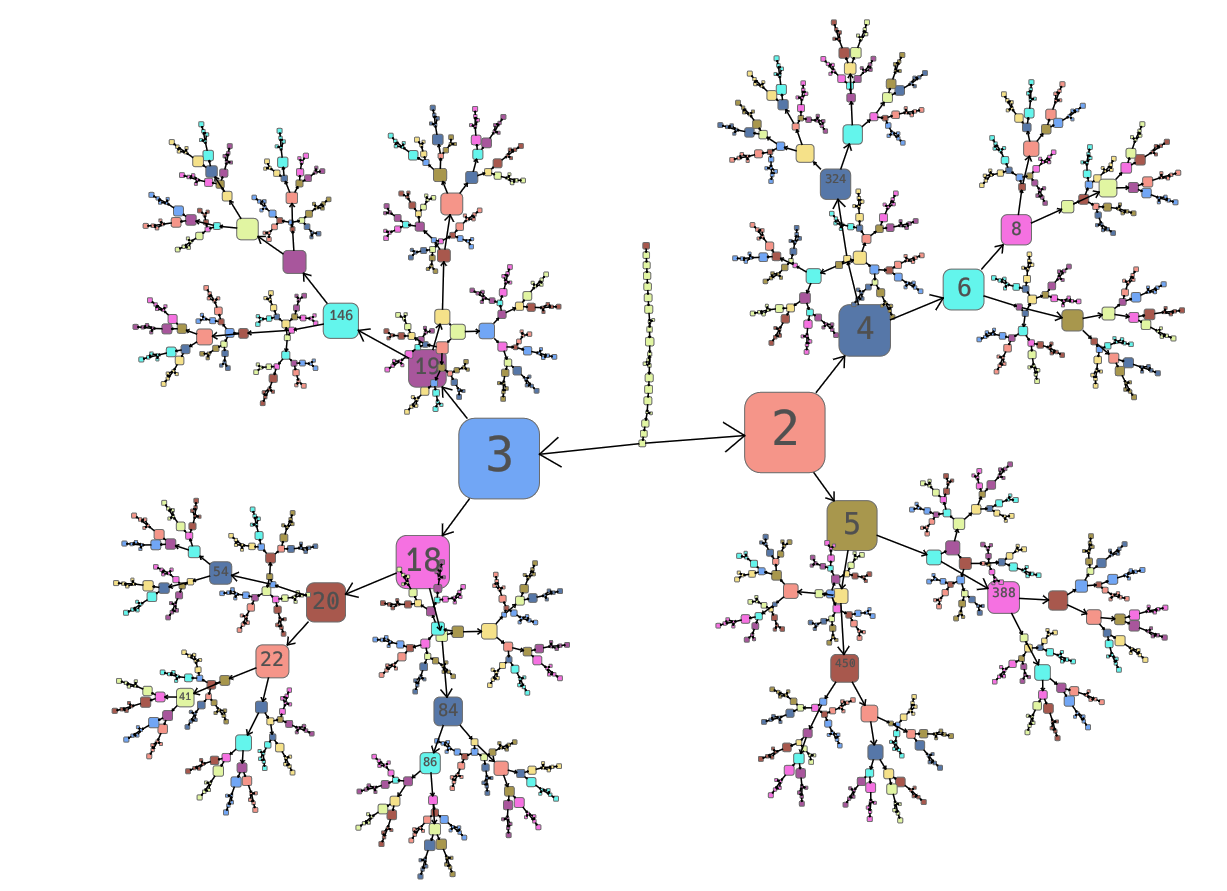
\includegraphics[width=0.95\textwidth]{assets/state-splitter-alpha.png}
    \end{center}
\end{frame}


% 4. (minut 5-6) Säga att vi gjort detta på maskinkodsnivå med S2E
\section{AMBA}


% 5. (minut 7-11) Demo med enklare, successivt mer komplicerade exempel
\begin{frame}
	\centering
	\huge
	DEMO
\end{frame}


% 6. (minut 12) Utvecklingspotential
\begin{frame}

	\centering
    AMBA is cool, but not useful for real programs

\end{frame}

\begin{frame}

	\centering
    AMBA is cool, but not (yet) useful for real programs

\end{frame}

\begin{frame}

    \textbf{Why is it cool?}
    \vspace{1.8mm}

    In general:

    \begin{itemize}

        \item \underline{Visualized} symbolic fuzzing $\rightarrow$ Human domain

        \item Visualized \underline{symbolic fuzzing} $\rightarrow$ Computer's
            domain

        \item Human $+$ Computer $\rightarrow$ More powerful analysis possible

    \end{itemize}

\end{frame}
\begin{frame}


    \textbf{Why is it cool?}
    \vspace{1.8mm}

    AMBA vs other tools:

    \begin{itemize}

        \item Very few other tools exist. We know of one targeting machine code
            (SymNav). None based on \stoe{}

        \item System virtualization within QEMU through \stoe{}
            \begin{itemize}

                \item Realistic execution environment

                \item Easily extended to multi-process analysis

                \item Maybe kernel, device drivers?

            \end{itemize}

        \item Higher performance ceiling

        \item Real time architecture. No batching

    \end{itemize}

    \pause
    BUT!

    \pause
    AMBA needs
    \begin{itemize}
        \item polish, quality-of-life features

        \item real-world testing \& feedback incorporated

    \end{itemize}

\end{frame}


% 7. (minut 13) Arbetsprocessen (bortförklara varför utveckingspotential finns)
% (ish vecka för vecka, med figur)
\begin{frame}
	\begin{columns}[t]
		\begin{column}{0.4\textwidth}
			\textbf{Plan}
			\begin{enumerate}
				\item Built \stoe{} week 2--4
				\item Prototyped functionality week 5--13
				\item Integrated in AMBA week 8--16
			\end{enumerate}
		\end{column}
		\begin{column}{0.4\textwidth}
			\textbf{Reality}
			\begin{enumerate}
				\item Built \stoe{} week 2--7
				\item Prototyped functionality week 6--8
				\item Functionality built directly in AMBA week 8--18
			\end{enumerate}
		\end{column}
	\end{columns}
	\textbf{Consequences}
	\begin{enumerate}

		\item Features abandoned after investing nontrivial effort (e.g.
		      \texttt{malloc}/\texttt{free} tracking)

		\item Features chosen for simplicity of implementation, not user
		      utility.

		\item No external user testing or feedback whatsoever.

	\end{enumerate}
\end{frame}


\end{document}
